\documentclass[
a4paper,
oneside,
halfparskip*,
normalheadings,
]
{scrbook}

\usepackage[english]{babel}
\usepackage[ansinew]{inputenc}
\usepackage{graphicx}
\usepackage{url}

\begin{document}

\title{HE853 Control Documentation}
\author{Thomas Ascher}
\maketitle
\tableofcontents
\mainmatter

\chapter{Introduction}

The HE853 Control project is dedicated to create a Windows SDK for the HE853 USB
dongle of the Home Easy home automation products since the vendor does not provide
one.

The SDK consists of GPL licensed tools and a LGPL licensed library that can be
used from other applications.

Out target audience are power users and software developers who whish to extend the
usage of the HE853 USB dongle beyond the limits of the vendor software.

Most information this project is based on was gathered through reverse engineering.
So not all details of the used communiation protocol are known and documented.

For more information about the Home Easy home automation products please refer to
the vendor page: \url{http://www.elro.eu/en/products/category/home_automation/home_easy/zenders2/pc_afstandsbediening_usb_dongle}

For more information and the latest packages please refer to the project page:
\url{http://he853control.sourceforge.net/}

\section{Prequesites}
For installation, usage and development Microsoft .NET Framework 2.0 has to be installed on
your system: \url{http://go.microsoft.com/fwlink/?LinkId=131000}




\chapter{Tools}

All tools are located in the installation directory. 

\section{Command Line Utility -- HE853.Util.exe}

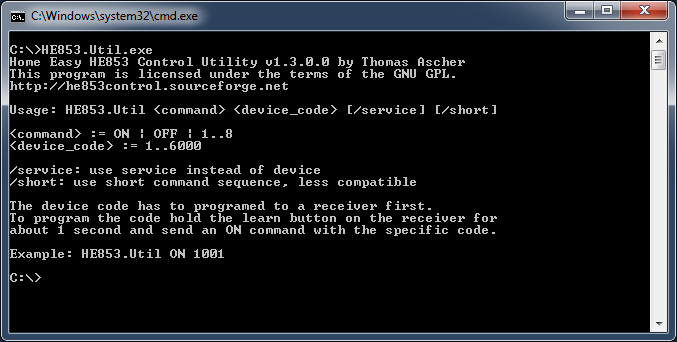
\includegraphics[width=300px]{cmd.png}

Usage: HE853.Util \textless command\textgreater \textless device\textunderscore code\textgreater [/service]

\textless command\textgreater := ON | OFF | 10..80
\textless device\textunderscore code\textgreater := 1..6000

Example: HE853.Util ON 1001

\section{GUI Application -- HE853.App.exe}

TODO

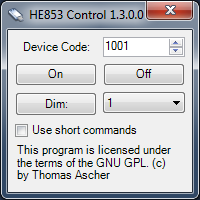
\includegraphics[width=100px]{gui.png}


\section{Coupling Dongle with Receivers}

Before a receiver react to commands of the USB dongle a specific device code has to be
programmed to the receiver first. A device code is a number between 1 and 6000 and can
be used by multiple receivers.

To program a device code use the command line utility or the GUI application. Press the
learn button on a receiver for about 1 second. Then send an ON command with the desired
device code from the command line utility or the GUI application. The receiver will
react to commands with this device code.

To clear the programmed device code press the learn button on a receiver util the LED
on the receiver starts to flash.

\section{Service -- HE853.Service.exe}

The service HE853.Service is for advanced users. It is meant for scenare where multiple
applications have to access the HE853 dongle concurrently. Both the utility and the
GUI application support the \textit{/service} switch that makes them use the service
instead of using the device directly.

TODO

\subsection{Configuration}

TODO

\subsection{Manual Installation}

TODO

If the service was not installed with the MSI installer

To install the service you have to use Installer Tool (Installutil.exe). The service is
configured to not start automatically per default. 




\chapter{Development}

For development at least Microsoft .NET Framework 2.0 and or Visual Studio 2005 is required.

\section{Using the Library -- HE853.dll}

The library can be used by any .NET language by referencing the HE853.dll assembly from the
installation directory or via COM. Please note that the assembly is compiled as Any CPU
and works with x86 and x64 platform configurations.

Visual Studio 2010 sample projects for the languages C++, C++/CLI, C\# and Visual Basic
are located in the installation folder in \textit{\textbackslash Samples}.

Please note that the library is licensed under the term of the LGPL. This means it is
possible to use the library in commercial applications but code changes to the library
have to be made available on distribution.

\subsection{C\# Sample Code}

\begin{verbatim}
HE853.IDevice device = new HE853.Device();
if (device.Open())
{
    device.On(1001);
    device.Off(1001);
    device.Close();
}
\end{verbatim}

\section{Using the RPC Library -- HE853.RPC.dll}

The RPC library ist not designed for general usage yet and is not available via COM.

\begin{verbatim}
HE853.RPC.RegisterClient();
HE853.IDevice device = new HE853.Device();
if (device.Open())
{
    device.On(1001);
    device.Off(1001);
    device.Close();
}
\end{verbatim}

\section{Depolyment}
The easiest method of depolyment is by installing the HE853 Control MSI setup on the target
system. The installation performs all required steps:

\begin{itemize}
  \item Installation of HE853.dll to the global assembly cache
	\item Registration of HE853.dll for COM usage
	\item Registration of HE853.Service.exe
\end{itemize}

If you deploy .NET applications you can simply install or copy the HE853.dll with your application
as private assembly.

\end{document}